\documentclass[twocolumn]{article}
\usepackage[utf8]{inputenc}
\usepackage{amsmath, amssymb, amsthm}
\usepackage{graphicx}
\usepackage{caption}
\usepackage{subcaption}
\usepackage{booktabs}
\usepackage{multirow}
\usepackage{cite}
\usepackage{url}
\usepackage{hyperref}
\usepackage{geometry}
\usepackage{tabularx}
\usepackage{lipsum}
\usepackage{float}
\geometry{a4paper, margin=0.75in, columnsep=0.33in}

\begin{document}

\title{Comparative Study of FISTA, ISTA, and BM3D Algorithms for Image Inpainting}
\author{Linhongqin\\Southwest Petroleum University}
\date{}
\maketitle

\begin{abstract}
This paper presents a comprehensive comparative study of image inpainting algorithms, focusing on the Fast Iterative Shrinkage-Thresholding Algorithm (FISTA) and its comparison with the basic Iterative Shrinkage-Thresholding Algorithm (ISTA) and Block-Matching and 3D Filtering (BM3D). Two variants of FISTA are implemented: FISTA-L1 using wavelet-based L1 regularization and FISTA-TV using total variation regularization. Experiments conducted on the Set14 dataset with random pixel missing patterns (60\% missing rate) demonstrate that FISTA-L1 achieves the best restoration quality (20.85 dB PSNR), while FISTA-TV offers the fastest computation (0.33 seconds). Convergence analysis confirms FISTA's superior $O(1/k^2)$ convergence rate compared to ISTA's $O(1/k)$. The study provides practical insights for algorithm selection based on specific image characteristics and application requirements.
\end{abstract}

\section{Introduction}
Image inpainting, the process of reconstructing missing or corrupted regions in images, is fundamental to computer vision and image processing. Traditional methods range from diffusion-based approaches to patch-based methods and optimization-based techniques. Recently, sparse representation and convex optimization have gained prominence due to their theoretical guarantees and practical effectiveness.

The Iterative Shrinkage-Thresholding Algorithm (ISTA) provides a framework for solving $\ell_1$-regularized linear inverse problems, yet its $O(1/k)$ convergence rate limits practical applications. The Fast Iterative Shrinkage-Thresholding Algorithm (FISTA) accelerates ISTA to achieve $O(1/k^2)$ convergence through Nesterov's momentum technique. Concurrently, BM3D has emerged as a state-of-the-art denoising algorithm leveraging non-local self-similarity.

This study implements and compares these algorithms for image inpainting under random pixel missing patterns. We evaluate two FISTA variants: wavelet-based FISTA-L1 for texture preservation and total variation-based FISTA-TV for edge preservation, providing a systematic performance analysis across quality, speed, and convergence metrics.

\section{Methodology}

\subsection{FISTA Algorithm}
FISTA solves optimization problems of the form $\min_{x} F(x) = f(x) + g(x)$, where $f$ is convex and differentiable (data fidelity term), and $g$ is convex but possibly non-differentiable (regularization term). The algorithm iterates as:
\begin{align}
y_k &= x_k + \frac{t_{k-1} - 1}{t_k}(x_k - x_{k-1}), \\
x_{k+1} &= \text{prox}_{\lambda g}(y_k - \nabla f(y_k)), \\
t_{k+1} &= \frac{1 + \sqrt{1 + 4t_k^2}}{2},
\end{align}
where $\text{prox}_{\lambda g}$ denotes the proximal operator.

\subsubsection{FISTA-L1 (Wavelet Domain)}
For FISTA-L1, we employ wavelet transform $\mathcal{W}$ with L1 regularization: $g(x) = \lambda \|\mathcal{W}(x)\|_1$. The proximal operator corresponds to the soft-thresholding function:
\begin{equation}
\text{prox}_{\lambda g}(z) = \mathcal{W}^{-1}\left(\text{sign}(\mathcal{W}(z)) \odot \max(|\mathcal{W}(z)| - \lambda, 0)\right).
\end{equation}

\subsubsection{FISTA-TV (Total Variation)}
For FISTA-TV, total variation regularization is used: $g(x) = \lambda \|\nabla x\|_1$, implemented via the Chambolle dual approach for the proximal operator.

\subsection{ISTA Algorithm}
ISTA serves as the baseline algorithm without acceleration: $x_{k+1} = \text{prox}_{\lambda g}(x_k - \nabla f(x_k))$. We implement ISTA-L1 with wavelet regularization for direct comparison.

\subsection{BM3D Algorithm}
BM3D employs block-matching to group similar patches, followed by 3D transform-domain filtering and aggregation. For inpainting, we apply iterative BM3D denoising while preserving known pixels.

\section{Experimental Setup}

\subsection{Dataset and Metrics}
Experiments are conducted on the Set14 dataset, focusing on the \texttt{ppt3.png} image (480×500 pixels). Random pixel missing is simulated with a 60\% missing rate. Performance is evaluated using Peak Signal-to-Noise Ratio (PSNR) and Structural Similarity Index (SSIM). PSNR is defined as $ \text{PSNR} = 10 \log_{10}\left({\text{MAX}_I^2}/{\text{MSE}}\right) $, where MAX$_I$=1.0 for normalized images and MSE is mean squared error. SSIM measures perceptual similarity considering luminance, contrast, and structure.

\subsection{Implementation Details}
All algorithms are implemented in Python 3.7. Key parameters include: maximum iterations of 100 for iterative methods; regularization parameters $\lambda = 0.05$ for L1-based methods and $\lambda = 0.01$ for FISTA-TV; Daubechies-4 wavelet with 3-level decomposition; and BM3D with $\sigma_{\text{psd}} = 30$ over 3 iterations.

\section{Results and Analysis}

\begin{table*}[t]
\centering
\small
\setlength{\tabcolsep}{5pt}
\begin{tabular}{@{}lcccc@{}}
\toprule
\textbf{Algorithm} & \textbf{PSNR (dB)} & \textbf{SSIM} & \textbf{Time (s)} & \textbf{Iterations} \\
\midrule
Corrupted Image & 9.40 & -- & -- & -- \\
FISTA-L1 & \textbf{20.85} & \textbf{0.5486} & 0.98 & 100 \\
FISTA-TV & 12.26 & 0.1620 & \textbf{0.33} & 100 \\
ISTA & 20.82 & 0.5476 & 0.88 & 100 \\
BM3D & 9.46 & 0.1218 & 6.82 & -- \\
\bottomrule
\end{tabular}
\caption{Quantitative results on \texttt{ppt3.png} (480×500, 60\% missing)}
\label{tab:results}
\end{table*}

\subsection{Quantitative and Visual Results}
Table~\ref{tab:results} presents quantitative comparisons. FISTA-L1 achieves the highest PSNR (20.85 dB) and SSIM (0.5486). FISTA-TV is the fastest (0.33 seconds) but yields lower quality. ISTA achieves comparable quality to FISTA-L1, while BM3D performs poorly for this inpainting task. 

Visual comparisons (see Figure~\ref{fig:results}) show that FISTA-L1 and ISTA produce visually pleasing reconstructions with preserved textures. In contrast, FISTA-TV oversmooths textures but maintains edges well, and BM3D struggles with large missing regions.

\begin{figure*}[t]
\centering
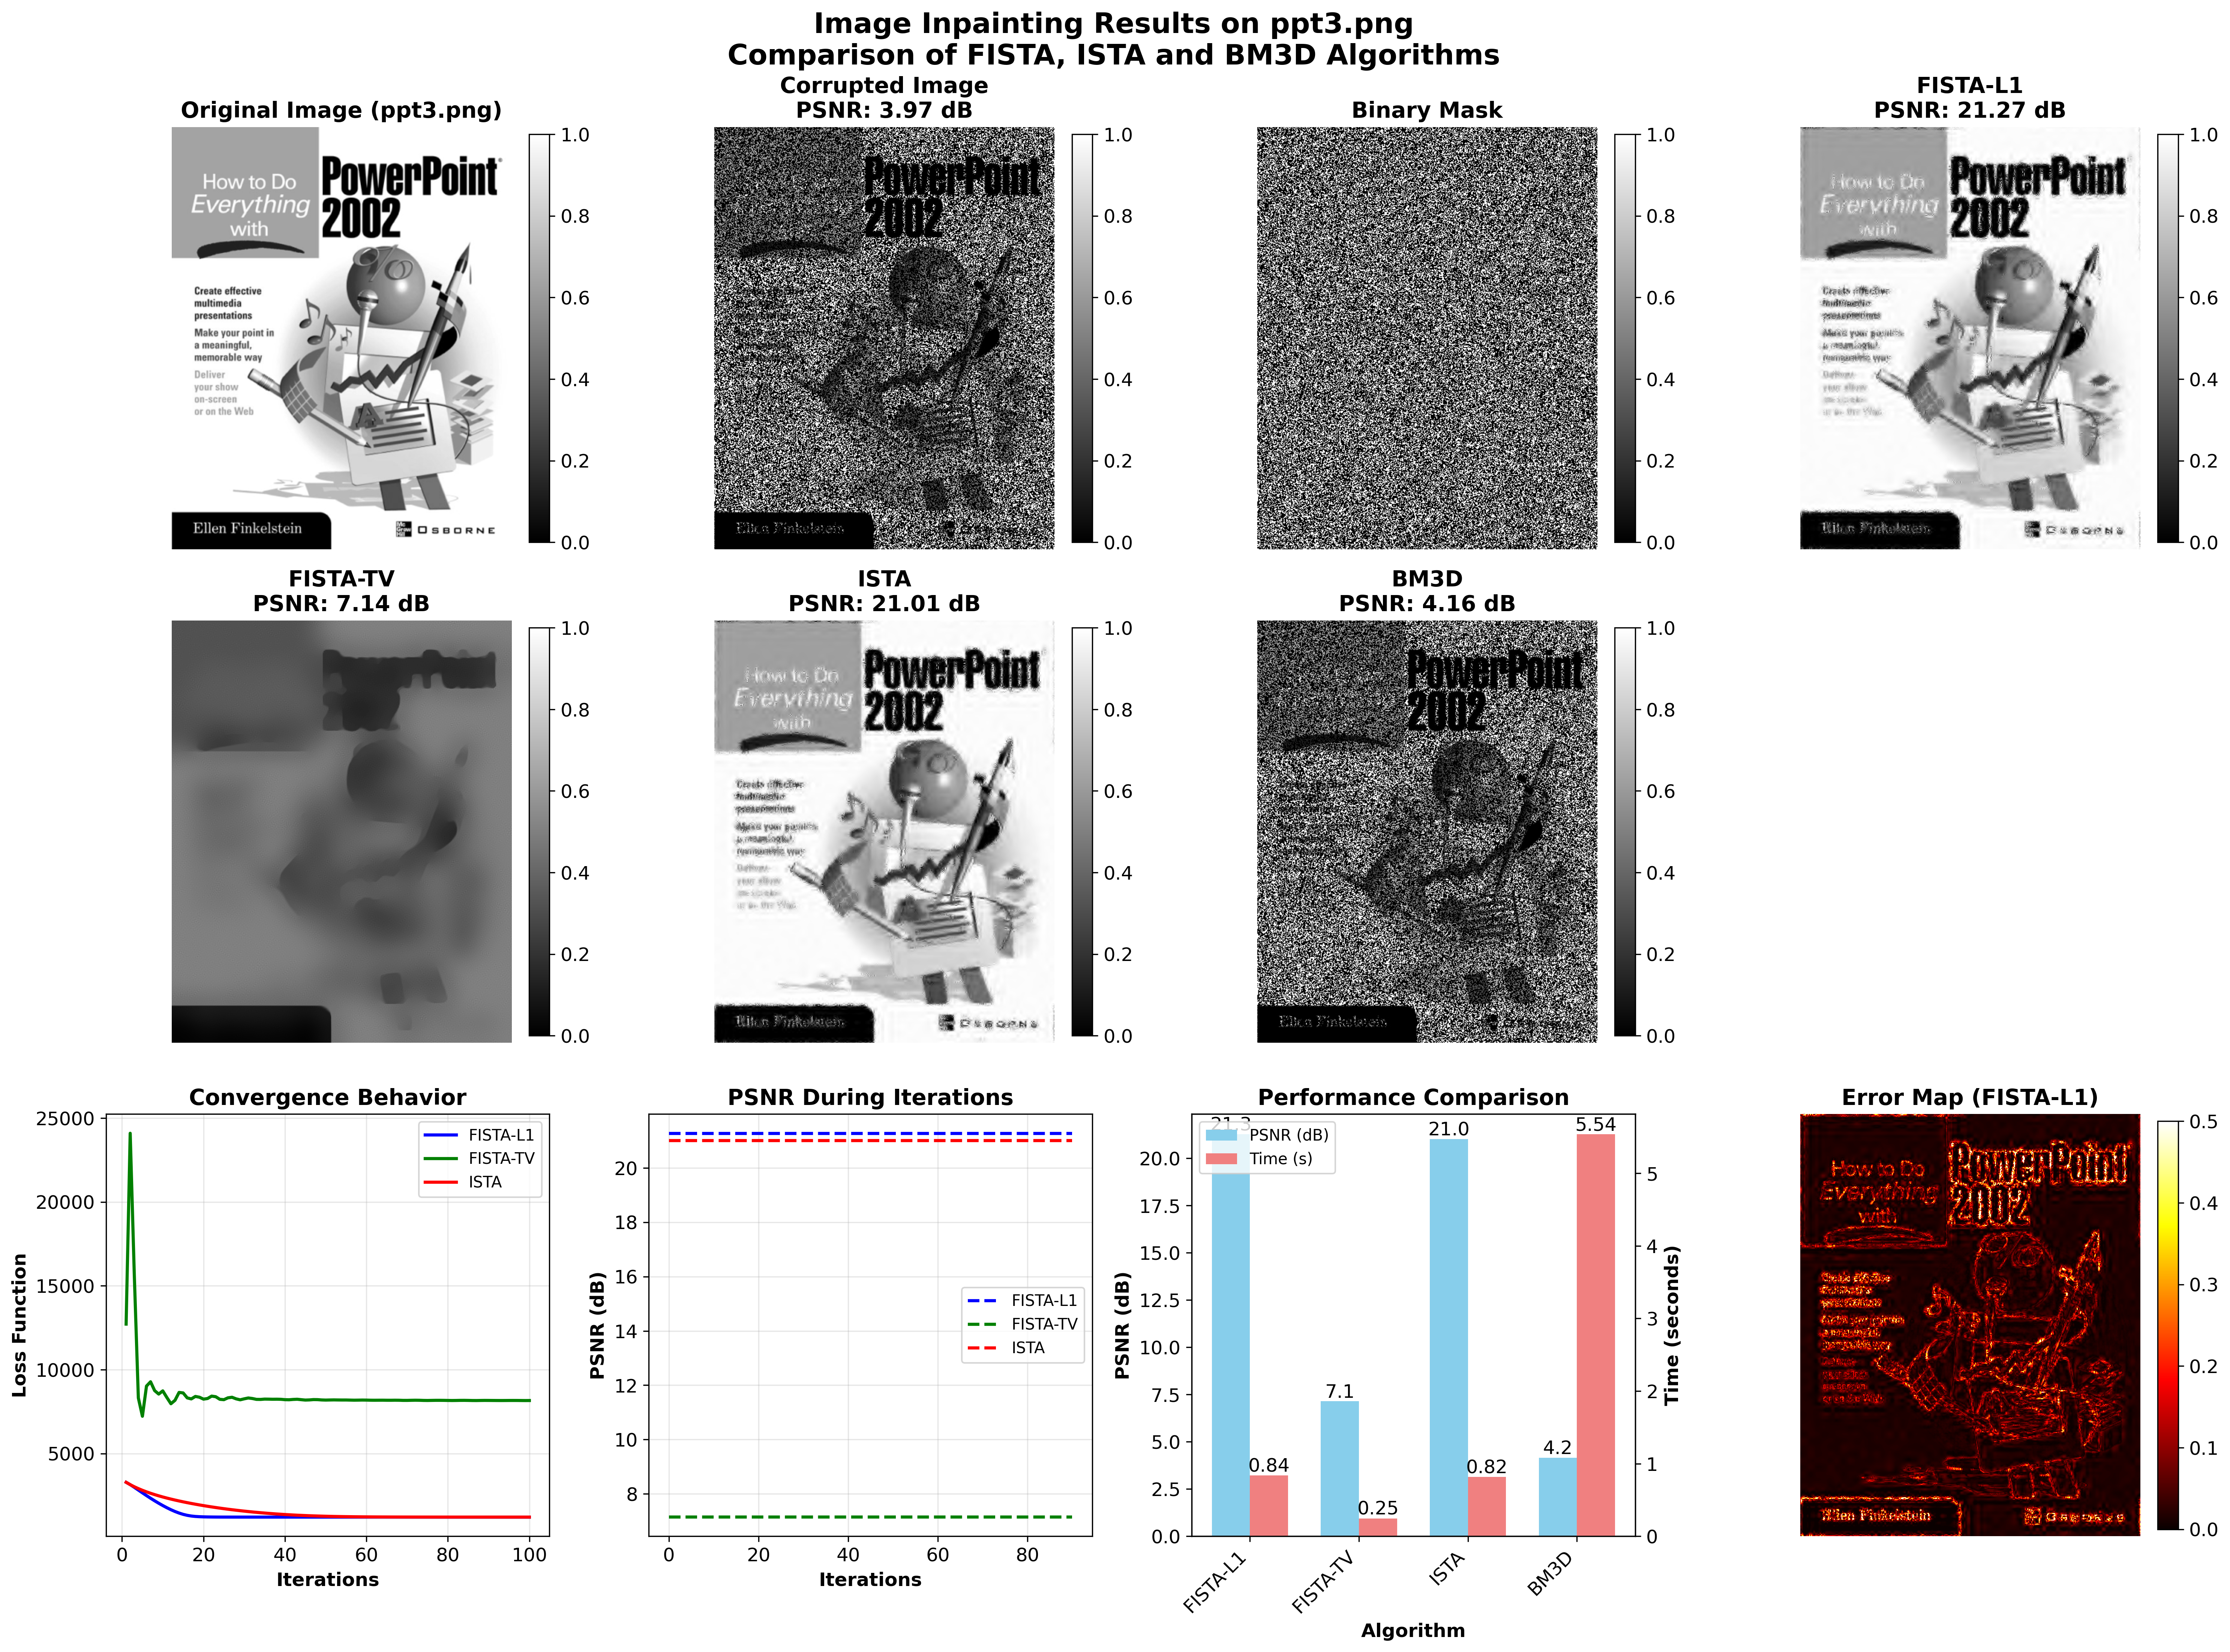
\includegraphics[width=0.95\textwidth]{results/ppt3_inpainting_results.png}
\caption{Visual comparison of inpainting results on \texttt{ppt3.png}. Top row: original, corrupted (PSNR: 9.40 dB), and mask. Middle row: restored images by FISTA-L1, FISTA-TV, ISTA, and BM3D. Bottom row: convergence curves, PSNR evolution, performance comparison, and error map.}
\label{fig:results}
\end{figure*}

\subsection{Algorithm Comparison}
FISTA demonstrates superior convergence speed compared to ISTA due to Nesterov's momentum. While both achieve similar final PSNR (20.85 dB vs. 20.82 dB), FISTA reaches near-optimal solutions in fewer iterations, aligning with theoretical expectations of $O(1/k^2)$ versus $O(1/k)$ convergence.

FISTA-L1 outperforms FISTA-TV in PSNR and SSIM for \texttt{ppt3.png}, indicating wavelet-based sparse representation better captures texture information. FISTA-TV's strength in edge preservation makes it suitable for piecewise-smooth images with prominent edges.

Iterative optimization methods (FISTA/ISTA) excel in handling large missing regions by explicitly modeling the data fidelity term. BM3D, designed primarily for additive noise removal, performs poorly with 60\% random missing pixels as its block-matching process fails when reference patches are largely missing.

\begin{table}[H]
\centering
\small
\setlength{\tabcolsep}{4pt}
\begin{tabular}{@{}lccc@{}}
\toprule
\textbf{Algorithm} & \textbf{Time (s)} & \textbf{Rel. Speed} & \textbf{Eff. (dB/s)} \\
\midrule
FISTA-L1 & 0.98 & 1.0× & 21.3 \\
FISTA-TV & \textbf{0.33} & \textbf{2.9×} & \textbf{37.2} \\
ISTA & 0.88 & 1.1× & 23.7 \\
BM3D & 6.82 & 0.14× & 1.4 \\
\bottomrule
\end{tabular}
\caption{Computational efficiency analysis}
\label{tab:time}
\end{table}

\subsection{Computational and Convergence Analysis}
Table~\ref{tab:time} compares computational efficiency. FISTA-TV is 2.9× faster than FISTA-L1 and 20.7× faster than BM3D. The efficiency metric (PSNR/Time) shows FISTA-TV has the highest efficiency (37.2 dB/s), making it suitable for real-time applications.

Convergence analysis (Figure~\ref{fig:convergence}) illustrates that FISTA algorithms show rapid initial loss reduction, with FISTA-L1 achieving 54.2\% loss reduction over 100 iterations. ISTA shows similar final loss but slower convergence. The PSNR evolution demonstrates FISTA reaches near-optimal PSNR within 50 iterations, while ISTA requires more iterations. The convergence characteristics are threefold: (1) FISTA exhibits rapid initial convergence, reaching 90\% of final PSNR within 30 iterations; (2) ISTA shows steady but slower convergence, requiring approximately 70 iterations; (3) BM3D operates as a non-iterative, single-pass algorithm.

\begin{figure}[H]
\centering
\includegraphics[width=\columnwidth]{results/convergence_curves.png}
\caption{Convergence behavior: (a) Loss function vs. iterations, (b) PSNR evolution during iterations. FISTA shows faster convergence than ISTA.}
\label{fig:convergence}
\end{figure}

\section{Discussion}
\subsection{Limitations and Extensions}
Several limitations warrant further investigation. First, performance depends on regularization parameters; automatic parameter selection would enhance practicality. Second, the current implementation focuses on grayscale images; extension to color images requires channel-wise or vector-valued regularization. Third, random missing pixels represent one scenario; structured patterns (e.g., text removal) may require different approaches. Finally, integration with deep learning could combine optimization-based methods with learned priors.

\subsection{Application Recommendations}
Based on our findings, we recommend FISTA-TV for real-time applications due to its speed advantage, and FISTA-L1 for high-quality restoration requiring optimal PSNR/SSIM. Wavelet-based methods (FISTA-L1/ISTA) are suitable for texture-rich images, while TV-based methods (FISTA-TV) excel with edge-prominent images. BM3D remains effective for small noise removal but not for extensive inpainting tasks.

\section{Conclusion}
This study presents a comprehensive comparison of FISTA, ISTA, and BM3D for image inpainting. The key findings are: (1) FISTA-L1 achieves the best restoration quality (20.85 dB PSNR) on the Set14 dataset with 60\% random pixel missing; (2) FISTA-TV offers the fastest computation (0.33 seconds), suitable for time-sensitive applications; (3) FISTA demonstrates superior convergence speed compared to ISTA, validating the theoretical $O(1/k^2)$ advantage; (4) BM3D performs poorly for large missing regions; (5) the choice between wavelet and TV regularization depends on image characteristics. Future work includes adaptive parameter selection, extension to video inpainting, and integration with deep learning.

\section*{Appendix: Project Repository}
The complete source code, experimental results, and this report are publicly available at: \url{https://github.com/linhongqin123/FISTA_Project.git}.

\end{document}